\documentclass[10pt,conference,compsocconf]{IEEEtran}

\usepackage{hyperref}
\usepackage{graphicx}	% For figure environment
\usepackage{placeins}
\usepackage{float}


\begin{document}
\title{Machine Learning Project II}

\author{
  Andres Montero, Elias Poroma, Jonas J\"aggi\\
  \textit{School of Computer and Communication Sciences, EPFL, Switzerland}
}

\maketitle

\begin{abstract}
We predict the mood of a tweet (positive or negative). 
We use GloVe word representation.
We use logarithmic regression as a baseline model.
We also use neural networks.
We pre-process the data to get even better results (?)
The best model is a neural network architecture which predicts N-Grams for groups of words.

\end{abstract}

\section{Introduction}



\section{Word Representation}

Words are represented as embeddings (representation of each word as a vector with n elements)

\subsection{Training our own word embeddings}
We use matrix factorization to get an embedidding matrix for our words based on the     co-occurece matrix of these words in the training tweets.
 
 \subsection{Using pre-trained word embeddings}
 We use an embedding matrix which was created by Standford university based on 2,6 Billion tweets in different languages. We filter out onl the words which occur at least 5 times in  our training datast.

\section{Baseline - Logarithmic regression}
We take the ean of the word vectors for each tweet. We then perform 

\begin{table}[H]
  \caption{Logarithmic regression - Accuracy on a validation set of 10'000 tweets}
  \label{tab:models}
\begin{tabular}{|l|l|l|l|}
\hline
\textbf{GloVe Dimensions}                                                              & \textbf{Our GloVe} & \textbf{Pretrained GloVe}     \\ \hline
\begin{tabular}[c]{@{}l@{}}25\end{tabular}               &    0.0        & \begin{tabular}[c]{@{}l@{}}0.0\end{tabular} \\ \hline
\begin{tabular}[c]{@{}l@{}}50\end{tabular}               &    0.0        & \begin{tabular}[c]{@{}l@{}}0.0\end{tabular} \\ \hline
\begin{tabular}[c]{@{}l@{}}100\end{tabular}               &    0.0        & \begin{tabular}[c]{@{}l@{}}0.0\end{tabular} \\ \hline
\begin{tabular}[c]{@{}l@{}}200\end{tabular}               &    0.0        & \begin{tabular}[c]{@{}l@{}}0.0\end{tabular} \\ \hline
\end{tabular}
\end{table}
 
Higher embedding dimensions seem to deliver better results. Pretrained GloVe outperforms our GloVe by far.

\section{Convolutional Neural Networks}
 \subsection{Network architecture}
 We have tried different network architecctures. 
 We train in mini-batches of size 1024 tweets.
 We can increase the dimensions of the network layers (see table below). Higher dimensions deliver better results, but increase computation time significantly. 

\begin{table}[H]
  \caption{Validation accuracy for different network architectures. Time per minibatch serves as an indicator for network complexity.}
  \label{tab:models}
\begin{tabular}{|l|l|l|l|}
\hline
\textbf{Network}                                                              & \textbf{Accuracy} & \textbf{Time per minibatch [ms]}     \\ \hline
\begin{tabular}[c]{@{}l@{}}Network 1\end{tabular}               &    0.0        & \begin{tabular}[c]{@{}l@{}}0.0\end{tabular} \\ \hline
\begin{tabular}[c]{@{}l@{}}Network 2\end{tabular}               &    0.0        & \begin{tabular}[c]{@{}l@{}}0.0\end{tabular} \\ \hline
\begin{tabular}[c]{@{}l@{}}Network 3\end{tabular}               &    0.0        & \begin{tabular}[c]{@{}l@{}}0.0\end{tabular} \\ \hline
\begin{tabular}[c]{@{}l@{}}Network 4 - 64 channels\end{tabular}               &    0.0        & \begin{tabular}[c]{@{}l@{}}0.0\end{tabular} \\ \hline
\begin{tabular}[c]{@{}l@{}}Network 4 - 128 channels\end{tabular}               &    0.0        & \begin{tabular}[c]{@{}l@{}}0.0\end{tabular} \\ \hline
\begin{tabular}[c]{@{}l@{}}Network 4 - 256 channels\end{tabular}               &    0.0        & \begin{tabular}[c]{@{}l@{}}0.0\end{tabular} \\ \hline
\begin{tabular}[c]{@{}l@{}}Network 4 - 1024 channels\end{tabular}               &    0.0        & \begin{tabular}[c]{@{}l@{}}0.0\end{tabular} \\ \hline
\end{tabular}
\end{table}

 \subsection{Measures against overfitting}
 We use L2 regularization for our network layerrs. In addition, wee can use dropout (explain dropout here).
 
\begin{figure}[H]
  \centering
  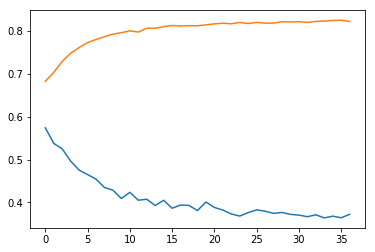
\includegraphics[width=\columnwidth]{overfitting}
  \caption{Evolution of Loss and Validation Accuracy}
  \vspace{-3mm}
  \label{fig:Validation accuracy vs Loss}
\end{figure}
 
 Dropout reduces the risk of overfitting, but in our case the tradeofff of having a less specific model is not worth it.
 

\section{Text Preprocesing}

We use different methods to preprocess text.


\begin{table}[H]
  \caption{Text preprocessing - Accuracy on a vlidation set of 10'000 tweets, using the NGrams network architecture}
  \label{tab:models}
\begin{tabular}{|l|l|l|l|}
\hline
\textbf{Preprocessing method}                                                              & \textbf{Accuracy}     \\ \hline
\begin{tabular}[c]{@{}l@{}}Method 1\end{tabular} & \begin{tabular}[c]{@{}l@{}}0.0\end{tabular} \\ \hline
\begin{tabular}[c]{@{}l@{}}Method 2\end{tabular} & \begin{tabular}[c]{@{}l@{}}0.0\end{tabular} \\ \hline
\begin{tabular}[c]{@{}l@{}}Method 3\end{tabular} & \begin{tabular}[c]{@{}l@{}}0.0\end{tabular} \\ \hline
\begin{tabular}[c]{@{}l@{}}Method 4\end{tabular} & \begin{tabular}[c]{@{}l@{}}0.0\end{tabular} \\ \hline
\end{tabular}
\end{table}

\section{Results and Summary}
Neural Networks offer a significative accuracy gain over logarithmic regression. Our implementations deliver consistent accuracy and are not much affected by overfitting. However, due to their computationa complexity special hardware is required for training them. Preprocessing the txt of the tweets allows us to increase accuracy even further (?). Achieving 100\% accuracy is not possible - some tweets don't express a clear emotion, and it is therefore impossible, even for a human, to guess the mood of it.
A detailed explanation of how to run the program is
in the ``README'' file presented with the results.


\bibliographystyle{IEEEtran}
\bibliography{literature}

\end{document}
